\section{Approach}
\label{sec:approach}

The ICQ framework, depicted in~\figref{fig:framework}, 
consists of three phases: data extraction, cue discovery, and model probing. 
In the data extraction phase, instances containing a 
specific linguistic feature $f$ are extracted from the dataset. 
The cue discovery phase identifies potential cues among pre-defined features. 
Finally, the model probing phase conducts two tests: 
the ``accuracy test'' and ``distribution test''. 
We will discuss these phases in more detail below.

\begin{figure}[th]
\centering
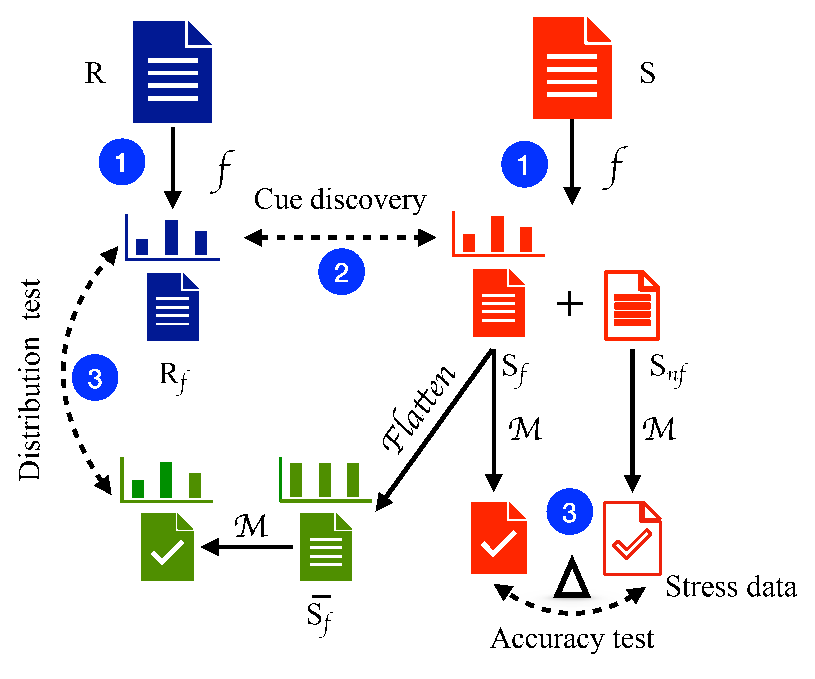
\includegraphics[width=0.6\columnwidth]{picture/framework.eps}
\caption{ICQ Workflow. \textcircled{1}: data extraction phase; \textcircled{2}: cue discovery phase; 
\textcircled{3}: model probing phase. $f$=a specific feature, $R$=training data, $S$=test data, $R_f$=extracted training data, 
$S_f$=extracted test data, $S_{nf}$=remaining test data without feature $f$, $\overline{S_f}$=flatten test data, $\mathcal{M}$=a sepecific model.}
\label{fig:framework}
\end{figure}


\subsection{Data Extraction Phase}
\label{sec:evaldata}
After defining the linguistic features, our system's fundamental step 
is constructing a data extractor for each feature value $f$. 
An extractor processes a dataset and retrieves a set of 
instances associated with the specified feature value. 
%For instance, in the ROCStories task, there is an extractor 
%for the word ``happy'' that retrieves all instances 
%containing ``happy'' in their endings, 
%including Example \ref{exp:roc}. 

\subsection{Cue Discovery Phase}
\label{sec:cuenessdiscovery}

For each feature $f$, we apply its extractor to both the 
training and test data of dataset $X$, 
denoted as $R$ and $S$ in \figref{fig:framework}. 
This results in clustered subsets of training 
instances ($R_f$) and test instances ($S_f$). 
A feature is considered a possible cue for a 
dataset only if it is present in both the training and test data.

The bias of the label distribution for an extracted set 
is computed using the mean squared error (MSE) 
and Jensen-Shannon Divergence (JSD)~\cite{lin1991divergence}. 
The cueness score indicates the extent 
to which dataset $X$ is biased against a feature $f$.

\begin{equation}
MSE(F) = \frac{1}{|L|} \sum_i (y_i - \overline{y_i})^2
\end{equation}

Here, $y_i$ represents the number of instances with label $l_i$ in the extracted dataset $F$, and $\overline{y_i}$ is the mean of $y_i$. A larger $MSE(F)$ implies a more pointed label distribution and greater bias. If the extracted training set and the extracted test set exhibit similar biases, 
the JSD between their distributions will be small:

\begin{equation}
JSD(R_f, S_f) = \frac{1}{2}\left (Q(R_f)\parallel A  \right )+\frac{1}{2}\left (Q(S_f)\parallel A  \right ), 
\end{equation}

where $ A = \frac{1}{2}\left (Q(R_f)+Q(S_f) \right )$. 
The function $Q()$ denotes the label distribution of the extracted dataset. We define the cueness score as:

\begin{equation}
cue(f, X) = \frac{MSE(R_f)}{\exp(JSD(R_f, S_f))}
\end{equation} 

This cueness score represents the degree to which a dataset $X$ is biased against a feature $f$.

\subsection{Model Probing Phase}
\label{sec:modelprobing}
In the previous section, we established that a dataset $X$ could be influenced by a cue $f$. However, a model trained on this dataset may not necessarily exploit that cue, as models depend on both data and architecture. In this section, we introduce a framework to probe any model instance trained on the biased dataset, assessing if it utilizes cue $f$ and to what degree. We achieve this through two tests: the \emph{accuracy test} and the \emph{distribution test}.

\subsubsection{Accuracy Test}
\label{sec:accuracytest}
The accuracy test examines the model's performance on data 
subsets with and without specific features. 
By comparing the model's accuracy on these two subsets, 
we can understand the model's generalization 
capabilities under different conditions. 
If the model's performance shows a noticeable improvement 
on the subset containing a specific feature, 
it may suggest that the model has exploited that feature for prediction.

In the accuracy test, we assess the prediction accuracies 
of the model $M$ on the extracted test set (with feature $f$) 
and on the remaining test set (without feature $f$), 
denoted as $acc(S_f)$ and $acc(S_{nf})$, respectively. 
The accuracy test computes the difference between these two accuracies:

\begin{equation}
\Delta Acc(f) = acc(S_f) - acc(S_{nf})
\end{equation}

A positive or negative value of 
$\Delta Acc$ indicates the direction of the model's performance 
change when comparing its accuracy on data subsets with 
and without specific features. A positive value 
suggests that the model exploits the feature for prediction, 
while a negative value implies struggles to 
generalize or detrimental sensitivity to the feature.

The magnitude of the absolute value of $\Delta Acc$ 
reflects the degree to which a model's performance 
is affected by the presence or absence 
of specific features in the data subsets. 
A larger absolute value indicates a 
stronger reliance on or sensitivity to the feature, 
whereas a smaller absolute value suggests a more 
robust model that is less affected by 
the presence or absence of the feature.


\subsubsection{Distribution Test}
\label{sec:distributiontest}
%Distribution test is a visual test. 
The distribution test is a visual examination that focuses 
on how changes in specific feature distributions 
within datasets affect a model's predictive performance.

First, we create a ``stress dataset'' $\overline{S_f}$ by 
``flattening'' the label distribution in $S_f$. 
We achieve this by removing random instances from all 
labels except for the one with the smallest number of instances, 
stopping when a balance is reached. In other words, 
we retain the minimum number of instances present in each label, 
while randomly discarding the excess instances. 
This approach effectively eliminates bias in the extracted test set, posing a challenge to the model.

Next, we apply the model to the stress test set 
and obtain prediction results. We then compare 
the label distribution of the prediction results 
on the stress test set with the label distribution 
of the extracted training data. The rationale is 
that if the extracted training data contains a cue, 
its label distribution will be skewed towards a specific label. 
If the model exploits this cue, it will prefer to predict that 
label as much as possible, amplifying the skewness of the distribution, 
despite the input test set being neutralized. 
We aim to observe such amplification in the 
output distribution to identify the model's weaknesses.

In summary, the accuracy test and distribution test are 
related in terms of assessing a model's sensitivity to 
specific features, but they emphasize different aspects. 
Distribution testing focuses on the impact of feature 
distribution changes on model performance, while accuracy 
testing evaluates the model's performance on data subsets 
with and without specific features. By combining these 
two testing methods, a model's sensitivity to particular 
features can be more comprehensively assessed. 
If both tests determine that the model is sensitive to 
a certain feature, we can have a higher degree of confidence in this conclusion.
